\documentclass{amsart}
\usepackage{amsmath, amssymb}
%\usepackage{mathpartir}
\usepackage{listings}
\usepackage{fancyvrb}
\usepackage{color}
\usepackage{bussproofs}
\usepackage{pgf, tikz}
\usepackage{graphicx}
\usetikzlibrary{arrows, automata}
\usepackage{hyperref}

\fvset{%
  fontsize=\small,
  numbers=left
}

\makeatletter
\renewcommand\subsection{\@startsection{subsection}{2}%
  \z@{-.5\linespacing\@plus-.7\linespacing}{.5\linespacing}%
  {\normalfont\scshape}}
\renewcommand\subsubsection{\@startsection{subsubsection}{3}%
  \z@{.5\linespacing\@plus.7\linespacing}{-.5em}%
  {\normalfont\scshape}}
\makeatother

\setcounter{tocdepth}{3}
\makeatletter
\def\l@subsection{\@tocline{2}{0pt}{2.5pc}{5pc}{}}
%Make Chapter disapear in ToC
\renewcommand\tocchapter[3]{%
  \indentlabel{\@ifnotempty{#2}{\ignorespaces#2.\quad}}#3%
}
\newcommand\@dotsep{4.5}
\def\@tocline#1#2#3#4#5#6#7{\relax
  \ifnum #1>\c@tocdepth % then omit
  \else
    \par \addpenalty\@secpenalty\addvspace{#2}%
    \begingroup \hyphenpenalty\@M
    \@ifempty{#4}{%
      \@tempdima\csname r@tocindent\number#1\endcsname\relax
    }{%
      \@tempdima#4\relax
    }%
    \parindent\z@ \leftskip#3\relax \advance\leftskip\@tempdima\relax
    \rightskip\@pnumwidth plus1em \parfillskip-\@pnumwidth
    #5\leavevmode\hskip-\@tempdima{#6}\nobreak
    \leaders\hbox{$\m@th\mkern \@dotsep mu\hbox{.}\mkern \@dotsep mu$}\hfill
    \nobreak
    \hbox to\@pnumwidth{\@tocpagenum{#7}}\par
    \nobreak
    \endgroup
  \fi}

\title{Git Instruction Manual}
\author{Evan Bergeron\\
Sunny Gakhar\\
Nishad Gothoskar\\
Frederick Lee\\
Ziyang Wang
}


\begin{document}
\maketitle

\tableofcontents
\newpage
\section*{Introduction}

This is a manual on how to set up Git on your computer and set up a basic Git workflow. The document covers installing and setting up Git and how to work with Git. The majority of this document is primarily intended for users who want to learn Git to use it in a fast-paced setting such as a hackathon, this document is also useful as a reference for experienced Git users who want to refer to some specifc concept or command which they need.

\section*{What is Git}

Git is a version control system designed to be used for working on small and large projects. It can be used for tracking changes between files and coordinating work on project files among multiple people.

\subsection*{Motivation}
When you were in school and you had short homework assignments, you would just start them and finish them in a short span of time (not longer than a week). But when you move on to designing and working on bigger projects with other people, there are multiple issues that come into play. Say you are participating in a hackathon and have finalized your idea and distribution of work among the teammates. How do you actually work on the project together? 

Having all of them work on one computer is not optimal. You might have each teammate work on his own piece independently, but how do you merge everyone's work? Moreover, what if two or more teammates work on the same file, but do different modifications unknown to the others? And what if someone wants to explore a different direction to work on, while keeping the original work intact? Enter Git.

\subsection*{Benefits}
\begin{enumerate}
  \item Using Git, if you're working on a project, you can "commit" the changes you have made and Git will keep track of all your commits. 
  
  \item If you want to explore a new direction of work which you don't want to integrate with your main project just yet, you can create a new branch and work on the branch without disturbing your main project. You can easily switch between multiple branches to work on multiple features, can when the time comes, you can merge with the main branch. 
\end{enumerate}

\newpage

\section*{Installing Git}

\subsection*{Windows}
If you have Windows, one easy way of installing Git is from this website:

\url{https://git-scm.com/download/win}

\noindent
Once you have downloaded the installation file, you can run it and proceed through the installation steps.

\subsection*{Mac}

Similar to Windows, one way of installing Git on is from this link

\url{https://git-scm.com/download/mac}


\noindent
Another way of installing Git is using the Xcode Command Line Tools. Open up Terminal 
and simply type \verb|git|. If you don’t have Git installed already, it will prompt you to install it.

\subsection*{Linux}

If you're working on Linux, you can install Git using a basic package management tool that comes with your distribution.

Debian/Ubuntu

\verb|$ apt-get install git|

\bigskip

Fedora

\verb|$ yum install git| (up to Fedora 21)

\verb|$ dnf install git| (Fedora 22 and later)

\bigskip

Arch Linux

\verb|$ pacman -S git|

\bigskip

FreeBSD

\verb|$ pkg install git|

\bigskip

Solaris 9/10/11 (OpenCSW)

\verb|$ pkgutil -i git|

\bigskip

Solaris 11 Express

\verb|$ pkg install developer/versioning/git|

\bigskip

OpenBSD

\verb|$ pkg_add git|


\newpage

\section*{Initializing Repository}

To make sure you have Git set up, type \verb|git| into your console (Terminal for Mac/Linux users and Command Prompt for Windows users) and the following should show up (the full output has been elided here).

\begin{verbatim}
$ git
usage: git [--version] [--help] [-C <path>] [-c name=value]
[--exec-path[=<path>]] [--html-path] [--man-path] [--info-path]
[-p | --paginate | --no-pager] [--no-replace-objects] [--bare]
[--git-dir=<path>] [--work-tree=<path>] [--namespace=<name>]
<command> [<args>]

...

'git help -a' and 'git help -g' list available subcommands and some
concept guides. See 'git help <command>' or 'git help <concept>'
to read about a specific subcommand or concept.
\end{verbatim}
\bigskip
\noindent
To start a new repository, first go to ttype \verb|git init| into the console. It should output the following:

\begin{verbatim}
$ git init
Initialized empty Git repository in <path to current directory>/.git/
\end{verbatim}

\bigskip
\noindent
This creates a \verb|./git| directory in your current directory, which consists of all information about the repository. It consists of a HEAD file, which points to the current version of the repository.


\newpage

\section*{Adding files to version control}

\section*{Committing changes}

\section*{Reverting changes}

\section*{Branching}

\section*{Merging Branches}

\newpage
\section*{Ignoring Files}

The best way to ignore files in a repository is to create a \texttt{.gitignore} file at the base of your repository with the names of all files to ignore.

Often you will find that in your projects, you will have files in your repository that do not need to be tracked.  These include automatically generated files, larger libraries that are really external dependencies, or system specific files such as the \texttt{.DS\_Store} file in Macs.

For example, let us have a repository with two files: \texttt{code.py} and \texttt{generated.txt}.  Here we only want to keep track of changes to \texttt{code.py} while ignoring changes to \texttt{generated.txt} which is automatically generated every time \texttt{code.py} is run.

Without a \texttt{.gitignore} file, running \texttt{git status} would get the following output:

\begin{verbatim}
$ git status
On branch master
Untracked files:
  (use "git add <file>..." to include in what will be committed)
  
    code.py
    generated.txt

nothing added to commit but untracked files present
(use "git add" to track)
\end{verbatim}

We create a \texttt{.gitignore} file with the following content:

\begin{verbatim}
generated.txt
.gitignore
\end{verbatim}

Running \texttt{git status} again, we see that the generated file and the \texttt{.gitignore} itself are ignored by Git as desired.

\begin{verbatim}
$ git status
On branch master
Untracked files:
  (use "git add <file>..." to include in what will be committed)
  
    code.py

nothing added to commit but untracked files present
(use "git add" to track)
\end{verbatim}

\newpage
\section*{Rebasing}

The rebasing and merging are the two primary ways of combining changes from separate branches with Git.  One primary advantage of rebasing is that the Git history is made more linear which makes it easier to track changes over time.

For example, say that you have been working on a separate branch called \texttt{feature} (shown in blue) on which you have two commits.  At the same time, a friend of yours has committed change ``C" to master (shown in green).

\begin{figure}[h]
\center
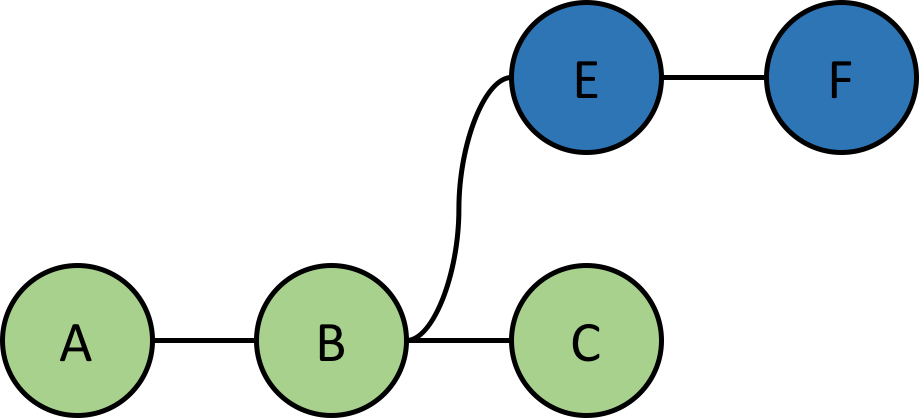
\includegraphics[height=2cm]{feature}
\end{figure}

A regular merge command such as
\begin{verbatim}
$ git checkout master
$ git merge feature
\end{verbatim}
would result in the following Git history:
\begin{figure}[h]
\center
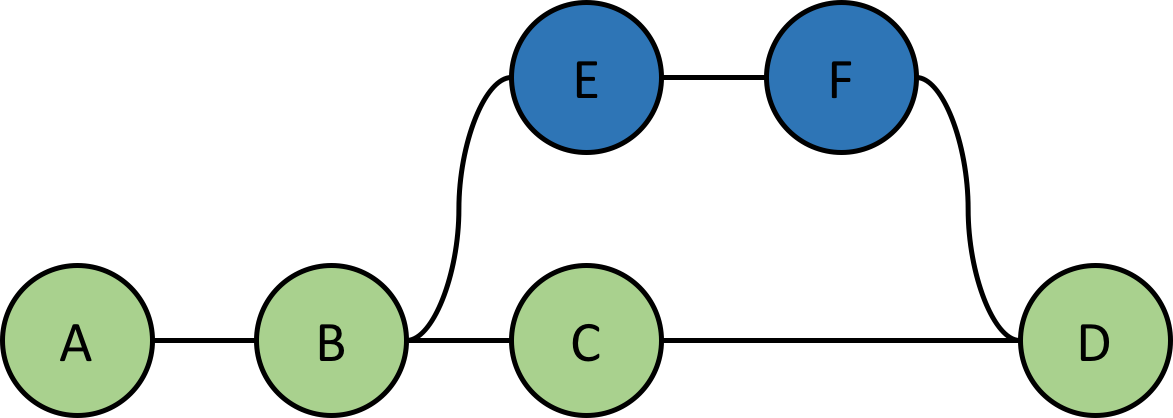
\includegraphics[height=2cm]{merge}
\end{figure}

However, if you want a more linear history, you would ideally want your commits ``E" and ``F" to be stacked on top of your friends commits.  To do as such, simply run as follows:
\begin{verbatim}
$ git checkout feature
$ git rebase master
$ git checkout master
$ git merge feature
\end{verbatim}

The initial rebase command changes the root of your \texttt{feature} branch to your friend's last commit as shown below on the left image.

\begin{figure}[h]
\center
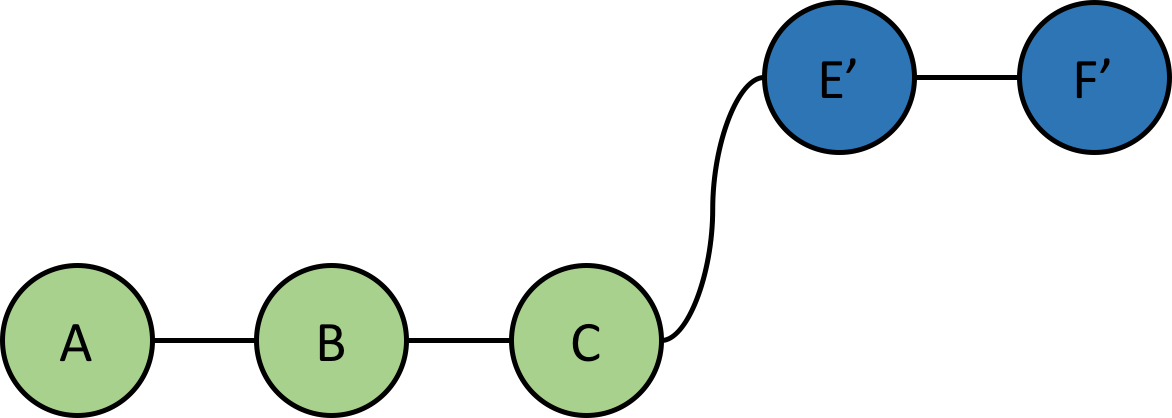
\includegraphics[height=2cm]{rebase}
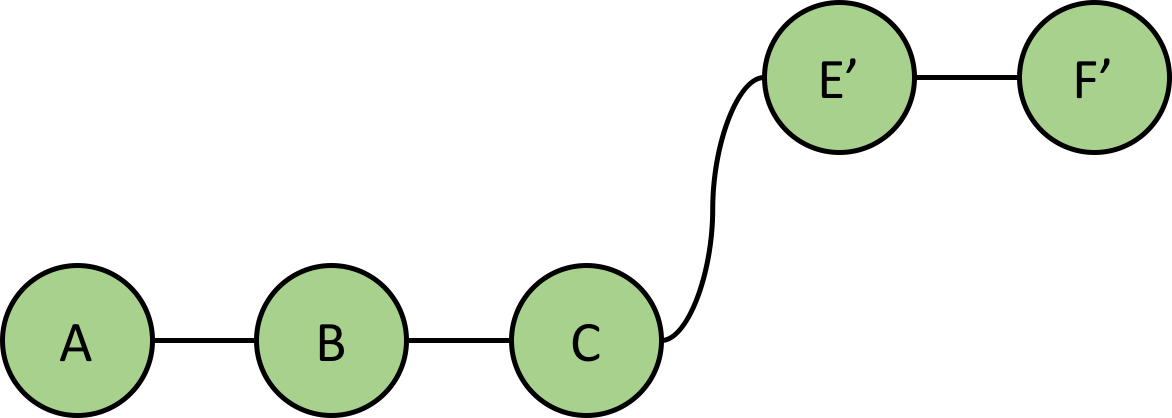
\includegraphics[height=2cm]{rebase_merge}
\end{figure}

The final merge of your feature onto master then forwards master's history to match your feature branch as shown above on the right.  As you can see, the history follows a much more linear pattern compared to the branching pattern of a regular merge alone.

\newpage
\section*{Cherry-picking}

Cherry-picking is particularly useful when you don't want to apply all changes from a branch to another branch through a merge or rebase, but only want to apply a few specific commits.

For example, take the hypothetical situation where your most recent commit ``F" in your feature branch (shown in blue) is suffering from a application-breaking bug, but your manager wants your changes in commit ``E" to be rolled out by this afternoon.

\begin{figure}[h]
\center
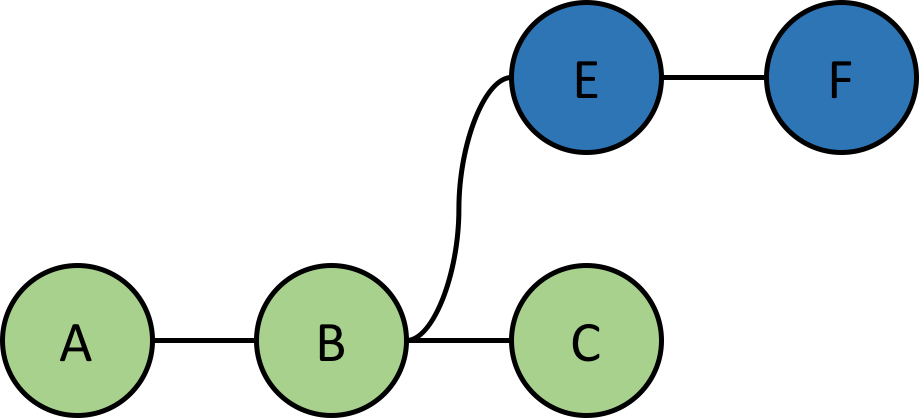
\includegraphics[height=2cm]{feature}
\end{figure}

To apply commit ``E" by itself to the master branch (in green), first find the commit-hash of your desired commit by running \texttt{git log} and searching for your commit.  A commit-hash is an identifying string of letters and numbers that may look something like \texttt{f3def414605008d5c899b2691ff1b6d1d3798a0a}.  After you have found your commit-hash, to apply your desired commit to the master branch, run the following commands:
\begin{verbatim}
$ git checkout master
$ git cherry-pick <commit-hash of E>
\end{verbatim}

Running these commands gets your final desired result shown below:

\begin{figure}[h]
\center
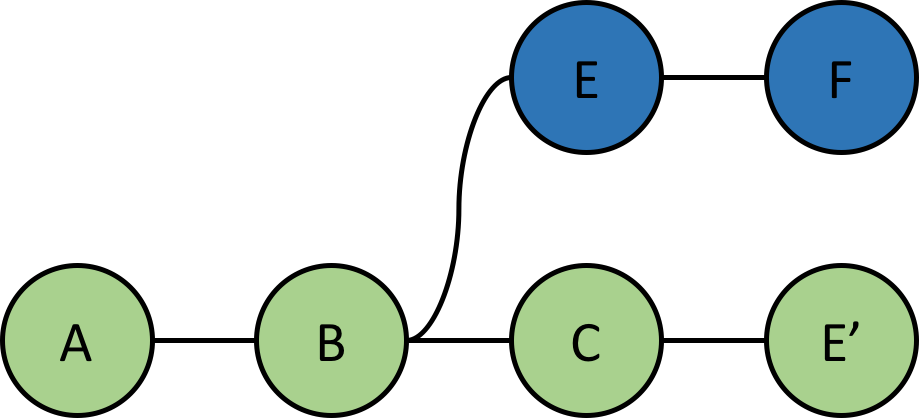
\includegraphics[height=2cm]{cherrypick}
\end{figure}

where commit ``E" has been applied to the master branch from your feature branch without merging your entire bug-ridden feature branch to master.

\newpage
\section*{Collaboration with Github}

\section*{General workflows}

\subsection*{Easily Reordering Commits}

We've all been there. You pull from master, take several minutes to
clean up the various merge conflicts, and then are ready to push. You
pull one last time before pushing, and what do you know - someone has
pushed again in the last couple minutes.

Previously, my workflow for this situation would look something like
\begin{verbatim}
$ git checkout -b tmp
$ git checkout master
$ git reset --hard HEAD~
$ git cherry-pick tmp
\end{verbatim}

This works fine, but there’s a much easier way -- one that involves
very little typing. We can simply say
\[
  \texttt{git rebase -i HEAD~2}
\]
This will open an interactive git rebasing session (the \texttt{-i}
stands for interactive). The window will display something along the
lines of
\begin{verbatim}
pick 370e221 Commit one
pick c342396 Commit two
\end{verbatim}
In whichever text editor we’re in, we may simply reorder these lines
to reorder the commits. Much shorter!

\subsection*{Adding partial files}
I just used this, actually. Suppose you’ve changed a single file
\texttt{foo.c} in different sections, and each of these changes are
logically different. For instance, maybe you refactor some function
\texttt{foo}, while at the same time fixing a bug in function
\texttt{bar}. Rather than create a separate branch and manually edit
the files, we can simply say
\[
  \texttt{git add -p foo.c}
\]
This will bring up an interactive prompt. It will automatically cycle
through all the different areas of the diff, asking you if you want to
stage each section. You may hit \texttt{y} or \texttt{n} for yes or
no.

Once you’re done adding the subset of changes you want to commit, you
can double-check you have the right changes staged by saying
\[
  \texttt{git diff --cached}
\]
Once you’re sure that you’re good to go, just commit your changes as
normal. You can repeat this process for the remaining changes. (Or
just do a normal \texttt{git add} at this point).

\subsection*{Git aliases}
Git aliases are a good way to save yourself a lot of typing. I
frequently want to see the git commit history, but don’t especially
care about the body of each commit. Here’s the command I’ve added to
my configuration:
\[
  \texttt{git config --global alias.l "log --oneline"}
\]
I can then just type “\texttt{git l}” to see a one line log of this
commit history. If there are several long commands you use frequently,
this can be a great way to save yourself some time.

\section*{Vim workflows}

At the time of writing, perhaps the most feature complete vim-git
plugin is Tim Pope’s “vim-fugitive.” Consequently, we will assume
usage of this plugin throughout the entire vim workflows tutorial.

\subsection*{Installing vim-fugitive}

There are a number of ways to install vim-fugitive. The one suggested
by Tim Pope is as follows:
\begin{verbatim}
$ cd ~/.vim/bundle
$ git clone git://github.com/tpope/vim-fugitive.git
$ vim -u NONE -c "helptags vim-fugitive/doc" -c q
\end{verbatim}
Vundle is a great plugin manager for vim -- if you use this, you may
simply add the line
\[
  \texttt{Plugin 'tpope/vim-fugitive}
\]
to your vimrc and run the \texttt{PluginInstall} command.

\subsection*{Easy git blame}
You’re browsing some file and discover a horrible bug written by one
of your coworkers. You’re about to storm over to someone’s desk and
verbally abuse them for producing incorrect code. Before you deliver
your diatribe, you need to know who to blame.

Before using \texttt{vim-fugitive}, you would have to exit vim,
manually type “\texttt{git blame <filename>},” and then search for the
relevant line in the output. Now, you can simply type
“\texttt{:Gblame}” in your vim prompt, and a vertical split will open
up right next to the line in question. You could even establish a
keybinding to do this for you! What was once several lines of typing
is now a single keystroke away! Your coworkers have never been so
scared\ldots

\section*{Emacs workflows}

Similarly to vim-fugitive for vim, “Magit” is (at the time of
writing), the most feature-complete git wrapper for emacs. We will
thus assume usage of this package.

\subsection*{Installing Magit}

\end{document}